%%%%% RESULTS %%%%%%
\section{Results}
\label{sec:results}

Figure \ref{fig:fidelity_plot} displays the haptic feedback fidelity and versatility scores of the systems described in each article. The quality score of each system is depicted by the dot's color and size, respectively (see section \ref{sec:confidence}).


\subsection{Search Results}

The search yielded 404 results, which were saved in the library of Mendeley. 75 duplicates were found and removed. The remaining 329 records were screened based on title and abstract first. This led to the preliminary exclusion of 290 records. Out of these, 73 records were re-screened as they were from the years 2022-2024, to better reflect the many recent advances in VR technology (see fig. \ref{fig:prisma}). 
Additionally, three papers were included based on citation search. 65 records were excluded during the re-screening process.

In total, 50 articles were found eligible for full-text screening. Of these, 14 were excluded based on the exclusion criteria, and the remaining 36 studies were included in this review.


\subsubsection{Study Characteristics}
\paragraph{Year of publication}
The included studies' publication dates from 2000 to 2024. As seen in figure \ref{fig:years}, the number of studies has greatly increased in the past decade, with a peak in 2019 and 2023. It must be noted, that this is partially due to the re-screening. 

\begin{figure}[htbp]
    \centering
    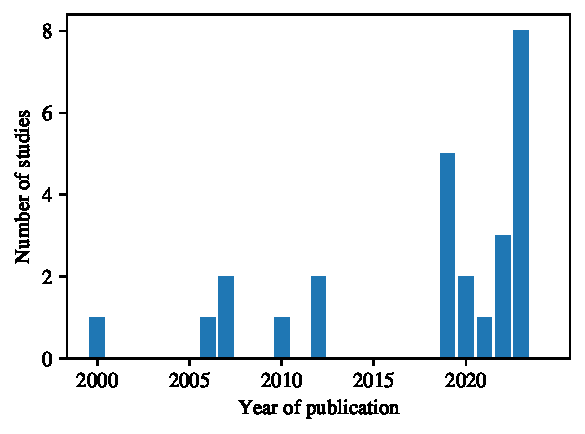
\includegraphics[width=\columnwidth]{figures/years.pdf} 
    \caption{Publication dates of the included articles}
    \label{fig:years}
\end{figure} 


\paragraph{Body Parts Involved}

Figure \ref{fig:body_parts_pie} shows which body parts were involved in the studies. As can be seen, most studies were concerned with stimuli at the palm and fingers, and many experiments also involved the forearm and upper arm. Two studies involved the feet, namely, the experiments utilizing the DaVinci Research Kit \cite{Caccianiga2021, Oquendo2024}.

\begin{figure}[htbp]
    \centering
    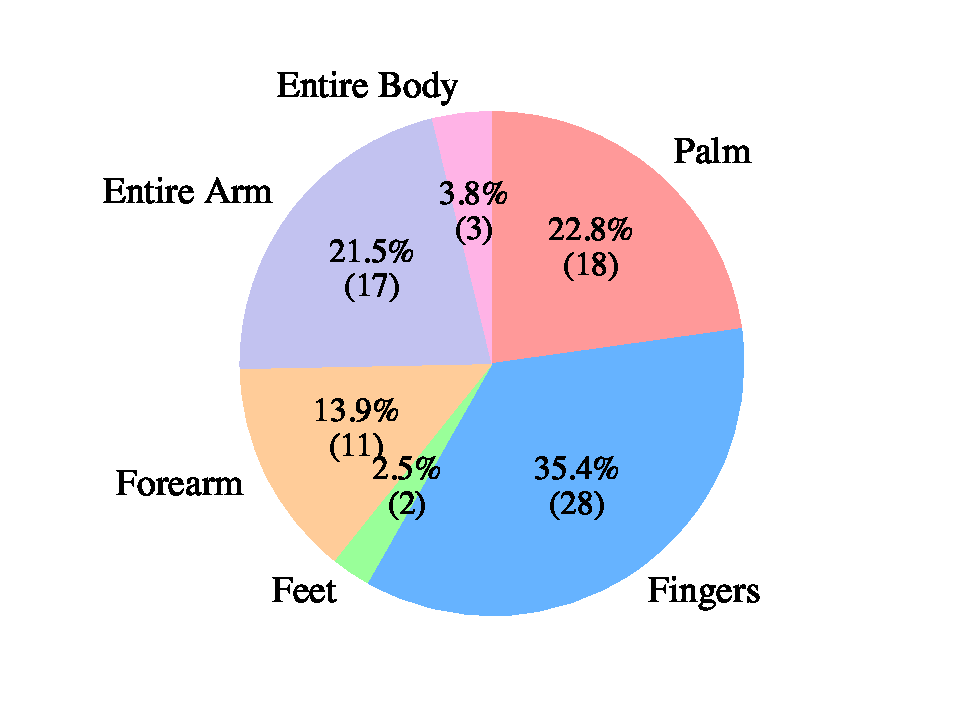
\includegraphics[width=\columnwidth]{figures/body_pie.pdf} 
    \caption{Body parts involved in the studies}
    \label{fig:body_parts_pie}
\end{figure} 

\subsection{Search Analysis Results}

\subsubsection{Clustering of the Data}
The papers were evaluated based on the haptic fidelity framework by Muender et al. \cite{Muender2022HapticReality} and plotted based on their haptic fidelity and versatility score as can be seen in figure \ref{fig:fidelity_plot}. The plot also shows the different confidence scores based on the quality of the papers. 

\begin{figure*}[htbp]
\begin{tikzpicture}[scale=3.9]
    
    % Add axis labels
    \foreach \x in {0,0.5,1,1.5,2} {
        \draw [very thin, lightgray](\x*2 cm, 0-0.05) -- (\x*2 cm, 2+0.05) node[anchor=north] {};
        \draw [very thin, lightgray](0-0.05,\x cm) -- (4+0.05,\x cm) node[anchor=east] {};
    }

    % Draw the horizontal & vertical dotted lines
    \draw[dashed, thick, dottedlines] (4/3,0) -- (4/3,2);
    \draw[dashed, thick, dottedlines] (8/3,0) -- (8/3,2);
    \draw[dashed, thick, dottedlines] (0,2/3) -- (4,2/3);
    \draw[dashed, thick, dottedlines] (0,4/3) -- (4,4/3);

    % Draw axes
    \draw[thick,<->] (0,1) -- (4,1) node[anchor=south west] {\parbox{2cm}{Haptic \\ Fidelity}};
    \draw[thick,<->] (2,0) -- (2,2) node[anchor=south] {Versatility};

    \node at (0,0.92) {\scriptsize{abstract}};
    \node at (2.3,0.92) {\scriptsize{representational}};
    \node at (4,0.92) {\scriptsize{realistic}};
    \node at (1.8,0.05) {\scriptsize{specific}};
    \node at (1.8,1.07) {\scriptsize{broad}};
    \node at (1.8,1.95) {\scriptsize{generic}};

    % Legend
    \draw[fill=white] (0.08,1.9) rectangle (1.16,1.25); % Legend border
    \node[anchor=west] at (0.12, 1.8) {\textbf{Legend}}; % Legend title
    
    \node[circle, fill=c1, inner sep=1.7pt] at (0.18, 1.65) {};
    \node[anchor=west] at (0.21, 1.65) {\scriptsize{Confidence $C > 0.9$}};

    \node[diamond, fill=c2, inner sep=1.3pt] at (0.18, 1.55) {};
    \node[anchor=west] at (0.21, 1.55) {\scriptsize{Confidence $0.8 < C \leq 0.9$}};

    \node[regular polygon, regular polygon sides=5, fill=c3, inner sep=1.7pt] at (0.18, 1.45) {};
    \node[anchor=west] at (0.21, 1.45) {\scriptsize{Confidence $0.7 < C \leq 0.8$}};

    \node[rectangle, fill=c4, inner sep=1.7pt] at (0.18, 1.35) {};
    \node[anchor=west] at (0.21, 1.35) {\scriptsize{Confidence $C \leq 0.7$}};


    % Sample data points
    \node[circle, fill=c1, inner sep=1.7pt] at (3.5,1) {};
    \node[circle, fill=c1, inner sep=1.7pt] at (3.22,1) {};
    \node[circle, fill=c1, inner sep=1.7pt] at (0.63,1) {};
    \node[circle, fill=c1, inner sep=1.7pt] at (3.01,1) {};
    \node[circle, fill=c1, inner sep=1.7pt] at (3.21,0.5) {};
    \node[circle, fill=c1, inner sep=1.7pt] at (3.38,1) {};
    \node[circle, fill=c1, inner sep=1.7pt] at (3.75,1) {};
    \node[circle, fill=c1, inner sep=1.7pt] at (2.63,1) {};
    \node[circle, fill=c1, inner sep=1.7pt] at (2.75,1) {};
    \node[circle, fill=c1, inner sep=1.7pt] at (3.21,0) {};
    \node[circle, fill=c1, inner sep=1.7pt] at (3.25,1) {};
    \node[circle, fill=c1, inner sep=1.7pt] at (4,0) {};
    \node[circle, fill=c1, inner sep=1.7pt] at (4,0.5) {};
    \node[circle, fill=c1, inner sep=1.7pt] at (3.88,0.5) {};
    \node[circle, fill=c1, inner sep=1.7pt] at (2.84,1.5) {};
    \node[circle, fill=c1, inner sep=1.7pt] at (3.7,0.5) {};
    \node[circle, fill=c1, inner sep=1.7pt] at (1.5,1.5) {};
    \node[circle, fill=c1, inner sep=1.7pt] at (2.57,2) {};
    \node[circle, fill=c1, inner sep=1.7pt] at (3.59,0.5) {};
    \node[circle, fill=c1, inner sep=1.7pt] at (2.72,1) {};
    \node[circle, fill=c1, inner sep=1.7pt] at (3.09,1) {};
    \node[circle, fill=c1, inner sep=1.7pt] at (3.5,1) {};
    \node[circle, fill=c1, inner sep=1.7pt] at (2.57,2) {};
    \node[diamond, fill=c2, inner sep=1.3pt] at (3.22,0.5) {};
    \node[diamond, fill=c2, inner sep=1.3pt] at (3.34,0.5) {};
    \node[diamond, fill=c2, inner sep=1.3pt] at (3.34,0.5) {};
    \node[diamond, fill=c2, inner sep=1.3pt] at (3.34,0.5) {};
    \node[diamond, fill=c2, inner sep=1.3pt] at (3.62,0.5) {};
    \node[diamond, fill=c2, inner sep=1.3pt] at (3.75,1) {};
    \node[diamond, fill=c2, inner sep=1.3pt] at (3.09,0.5) {};
    \node[diamond, fill=c2, inner sep=1.3pt] at (3.71,0.5) {};
    \node[diamond, fill=c2, inner sep=1.3pt] at (3.29,1) {};
    \node[diamond, fill=c2, inner sep=1.3pt] at (2.28,0.5) {};
    \node[diamond, fill=c2, inner sep=1.3pt] at (2.99,1.5) {};
    \node[diamond, fill=c2, inner sep=1.3pt] at (3.42,1.5) {};
    \node[diamond, fill=c2, inner sep=1.3pt] at (2.76,0.5) {};
    \node[diamond, fill=c2, inner sep=1.3pt] at (3.71,1) {};
    \node[diamond, fill=c2, inner sep=1.3pt] at (2.63,2) {};
    \node[diamond, fill=c2, inner sep=1.3pt] at (2.84,1) {};
    \node[diamond, fill=c2, inner sep=1.3pt] at (3.27,1) {};
    \node[regular polygon, regular polygon sides=5, fill=c3, inner sep=1.7pt] at (2.2,1) {};
    \node[regular polygon, regular polygon sides=5, fill=c3, inner sep=1.7pt] at (2.8,1) {};
    \node[regular polygon, regular polygon sides=5, fill=c3, inner sep=1.7pt] at (1.25,1.5) {};
    \node[regular polygon, regular polygon sides=5, fill=c3, inner sep=1.7pt] at (1.08,0.5) {};
    \node[regular polygon, regular polygon sides=5, fill=c3, inner sep=1.7pt] at (1.39,1) {};
    \node[regular polygon, regular polygon sides=5, fill=c3, inner sep=1.7pt] at (2.49,1.5) {};
    \node[regular polygon, regular polygon sides=5, fill=c3, inner sep=1.7pt] at (3.61,0) {};
    \node[regular polygon, regular polygon sides=5, fill=c3, inner sep=1.7pt] at (2.31,1.5) {};
    \node[rectangle, fill=c4, inner sep=1.7pt] at (4,0.5) {};


    % Add citations to datapoints
    \node at (3.5,1.1) {\footnotesize{\cite{Brickler2019}}};
    \node at (3.22,1.1) {\footnotesize{\cite{Caccianiga2021}}};
    \node at (0.63,1.1) {\footnotesize{\cite{Crespo2015}}};
    \node at (3.01,1.1) {\footnotesize{\cite{Dai2023}}};
    \node at (3.16,0.4) {\footnotesize{\cite{Dai2023}}};
    \node at (3.38,0.9) {\footnotesize{\cite{Feygin2002HapticSkill}}};
    \node at (3.75,1.2) {\footnotesize{\cite{Feygin2002HapticSkill}}};
    \node at (2.63,1.1) {\footnotesize{\cite{Gambaro2014}}};
    \node at (2.75,0.9) {\footnotesize{\cite{Gambaro2014}}};
    \node at (3.21,0.1) {\footnotesize{\cite{Graham2008}}};
    \node at (3.25,0.9) {\footnotesize{\cite{Gunter2022}}};
    \node at (4,0.1) {\footnotesize{\cite{Huang2006}}};
    \node at (4,0.6) {\footnotesize{\cite{Huang2007}}};
    \node at (3.88,0.6) {\footnotesize{\cite{LeeH2014}}};
    \node at (2.84,1.6) {\footnotesize{\cite{LeeY2019}}};
    \node at (3.7,0.6) {\footnotesize{\cite{LiuG2014}}};
    \node at (1.5,1.6) {\footnotesize{\cite{LiuH2019}}};
    \node at (2.57,2.1) {\footnotesize{\cite{McAnally2023}}};
    \node at (3.59,0.6) {\footnotesize{\cite{Mohanty2023}}};
    \node at (2.72,1.2) {\footnotesize{\cite{Oquendo2024}}};
    \node at (3.09,0.9) {\footnotesize{\cite{Oquendo2024}}};
    \node at (3.5,1.2) {\footnotesize{\cite{Rodriguez2010}}};
    \node at (2.57,1.9) {\footnotesize{\cite{Vasudevan2020}}};
    \node at (3.22,0.6) {\footnotesize{\cite{Fehlberg2012}}};
    \node at (3.285,0.4) {\footnotesize{\cite{Fehlberg2012}}};
    \node at (3.395,0.4) {\footnotesize{\cite{Fehlberg2012}}};
    \node at (3.34,0.6) {\footnotesize{\cite{Fehlberg2012}}};
    \node at (3.62,0.4) {\footnotesize{\cite{Fehlberg2012}}};
    \node at (3.75,1.1) {\footnotesize{\cite{Fehlberg2012}}};
    \node at (3.09,0.6) {\footnotesize{\cite{Grant2019}}};
    \node at (3.71,0.7) {\footnotesize{\cite{Macuga2019}}};
    \node at (3.35,1.1) {\footnotesize{\cite{Morris2007}}};
    \node at (2.28,0.6) {\footnotesize{\cite{Najdovski2020}}};
    \node at (2.99,1.6) {\footnotesize{\cite{Oezen2022}}};
    \node at (3.42,1.6) {\footnotesize{\cite{Oezen2022}}};
    \node at (2.76,0.6) {\footnotesize{\cite{Vaghela2021}}};
    \node at (3.71,0.9) {\footnotesize{\cite{Wall2000}}};
    \node at (2.7,2.1) {\footnotesize{\cite{Yang2023}}};
    \node at (2.84,1.2) {\footnotesize{\cite{Yang2023}}};
    \node at (3.27,1.2) {\footnotesize{\cite{Yang2023}}};
    \node at (2.2,1.1) {\footnotesize{\cite{Chappell2022}}};
    \node at (2.8,1.1) {\footnotesize{\cite{Chi2017}}};
    \node at (1.25,1.6) {\footnotesize{\cite{Hanashima2023}}};
    \node at (1.08,0.6) {\footnotesize{\cite{Lee2012}}};
    \node at (1.39,1.1) {\footnotesize{\cite{Perez2023}}};
    \node at (2.49,1.6) {\footnotesize{\cite{Trinitatova2023}}};
    \node at (3.61,0.1) {\footnotesize{\cite{Vaghela2021}}};
    \node at (2.31,1.6) {\footnotesize{\cite{Xia2023}}};
    \node at (4,0.4) {\footnotesize{\cite{Manivannan2008}}};
    
        
\end{tikzpicture}
\caption{Haptic fidelity and versatility scores for the included papers}
\label{fig:fidelity_plot}
\end{figure*}

As shown in figure \ref{fig:fidelity_plot}, the data is separated into 9 equally sized clusters, which are evaluated in section \ref{sec:evaluation_clusters}.


\subsubsection{Impact on Motor Learning}
The papers were evaluated based on the impact of the haptic feedback on motor learning (see section \ref{sec:impact_motor_learning}) and displayed in figure \ref{fig:motorlearning_plot}.

\begin{figure*}[htbp]
\begin{tikzpicture}[scale=3.9]

    % Draw axes
    \foreach \x in {0,0.5,1,1.5,2} {
        \draw [very thin, lightgray](\x*2 cm, 0-0.05) -- (\x*2 cm, 2+0.05) node[anchor=north] {};
        \draw [very thin, lightgray](0-0.05,\x cm) -- (4+0.05,\x cm) node[anchor=east] {};
    }

    % Add axis labels
    \draw[thick,<->] (0,1) -- (4,1) node[anchor=south west] {\parbox{2cm}{Haptic \\ Fidelity}};
    \draw[thick,<->] (2,0) -- (2,2) node[anchor=south] {Versatility};

    \node at (0,0.92) {\footnotesize{abstract}};
    \node at (2.3,0.92) {\scriptsize{representational}};
    \node at (4,0.92) {\footnotesize{realistic}};
    \node at (1.8,0.05) {\footnotesize{specific}};
    \node at (1.8,1.07) {\footnotesize{broad}};
    \node at (1.8,1.95) {\footnotesize{generic}};

    % Draw the horizontal & vertical dotted lines
    \draw[dashed, thick, dottedlines] (4/3,0) -- (4/3,2);
    \draw[dashed, thick, dottedlines] (8/3,0) -- (8/3,2);
    \draw[dashed, thick, dottedlines] (0,2/3) -- (4,2/3);
    \draw[dashed, thick, dottedlines] (0,4/3) -- (4,4/3);


    % Legend
    \draw[fill=white] (0.1,1.96) rectangle (0.97,1.2); % Legend border
    \node[anchor=west] at (0.13, 1.85) {\textbf{Legend}}; % Legend title
    
    \node[circle, fill=c1, inner sep=1.7pt] at (0.2, 1.73) {};
    \node[anchor=west] at (0.25, 1.73) {\scriptsize{Motor learning ++}};

    \node[diamond, fill=c2, inner sep=1.5pt] at (0.2, 1.65) {};
    \node[anchor=west] at (0.25, 1.65) {\scriptsize{Motor learning +}};

    \node[regular polygon, regular polygon sides=5, fill=c3, inner sep=1.5pt] at (0.2, 1.57) {};
    \node[anchor=west] at (0.25, 1.57) {\scriptsize{Motor learning o}};

    \node[rectangle, fill=c4, inner sep=1.7pt] at (0.2, 1.49) {};
    \node[anchor=west] at (0.25, 1.49) {\scriptsize{Motor learning -}};

    \node[star, star points=5, star point ratio=0.6, fill=c5, inner sep=1.6pt] at (0.2, 1.41) {};
    \node[anchor=west] at (0.25, 1.41) {\scriptsize{Motor learning - -}};

    \node[diamond, fill=c2, inner sep=1.2pt] at (0.2, 1.31) {};
    \node[diamond, fill=white, inner sep=0.5pt] at (0.2,1.31) {};
    \node[anchor=west] at (0.25, 1.31) {\scriptsize{Assumed value}};


    % Data Points
    \node[circle, fill=c1, inner sep=1.7pt] at (3.21,0.5) {};
    \node[circle, fill=c1, inner sep=1.7pt] at (3.01,1) {};
    \node[circle, fill=c1, inner sep=1.7pt] at (3.75,1) {};
    \node[circle, fill=c1, inner sep=1.7pt] at (3.62,0.5) {};
    \node[circle, fill=c1, inner sep=1.7pt] at (3.34,0.5) {};
    \node[circle, fill=c1, inner sep=1.7pt] at (3.09,0.5) {};
    \node[circle, fill=c1, inner sep=1.7pt] at (4,0) {};
    \node[circle, fill=c1, inner sep=1.7pt] at (1.5,1.5) {};
    \node[circle, fill=c1, inner sep=1.7pt] at (2.63,2) {};
    \node[circle, fill=c1, inner sep=1.7pt] at (3.27,1) {};
    \node[diamond, fill=c2, inner sep=1.2pt] at (3.5,1) {};
    \node[diamond, fill=c2, inner sep=1.2pt] at (3.22,1) {};
    \node[diamond, fill=c2, inner sep=1.2pt] at (2.2,1) {};
    \node[diamond, fill=c2, inner sep=1.2pt] at (2.8,1) {};
    \node[diamond, fill=c2, inner sep=1.2pt] at (3.34,0.5) {};
    \node[diamond, fill=c2, inner sep=1.2pt] at (3.34,0.5) {};
    \node[diamond, fill=c2, inner sep=1.2pt] at (3.22,0.5) {};
    \node[diamond, fill=c2, inner sep=1.2pt] at (2.63,1) {};
    \node[diamond, fill=c2, inner sep=1.2pt] at (2.75,1) {};
    \node[diamond, fill=c2, inner sep=1.2pt] at (3.21,0) {};
    \node[diamond, fill=c2, inner sep=1.2pt] at (3.25,1) {};
    \node[diamond, fill=c2, inner sep=1.2pt] at (4,0.5) {};
    \node[diamond, fill=c2, inner sep=1.2pt] at (3.88,0.5) {};
    \node[diamond, fill=c2, inner sep=1.2pt] at (2.84,1.5) {};
    \node[diamond, fill=c2, inner sep=1.2pt] at (3.7,0.5) {};
    \node[diamond, fill=c2, inner sep=1.2pt] at (3.71,0.5) {};
    \node[diamond, fill=c2, inner sep=1.2pt] at (4,0.5) {};
    \node[diamond, fill=c2, inner sep=1.2pt] at (2.57,2) {};
    \node[diamond, fill=c2, inner sep=1.2pt] at (3.59,0.5) {};
    \node[diamond, fill=c2, inner sep=1.2pt] at (2.28,0.5) {};
    \node[diamond, fill=c2, inner sep=1.2pt] at (3.42,1.5) {};
    \node[diamond, fill=c2, inner sep=1.2pt] at (2.72,1) {};
    \node[diamond, fill=c2, inner sep=1.2pt] at (3.5,1) {};
    \node[diamond, fill=c2, inner sep=1.2pt] at (2.49,1.5) {};
    \node[diamond, fill=c2, inner sep=1.2pt] at (3.61,0) {};
    \node[diamond, fill=c2, inner sep=1.2pt] at (2.57,2) {};
    \node[diamond, fill=c2, inner sep=1.2pt] at (3.71,1) {};
    \node[diamond, fill=c2, inner sep=1.2pt] at (2.31,1.5) {};
    \node[diamond, fill=c2, inner sep=1.2pt] at (2.84,1) {};
    \node[regular polygon, regular polygon sides=5, fill=c3, inner sep=1.3pt] at (0.63,1) {};
    \node[regular polygon, regular polygon sides=5, fill=c3, inner sep=1.3pt] at (1.25,1.5) {};
    \node[regular polygon, regular polygon sides=5, fill=c3, inner sep=1.3pt] at (3.38,1) {};
    \node[regular polygon, regular polygon sides=5, fill=c3, inner sep=1.3pt] at (3.75,1) {};
    \node[regular polygon, regular polygon sides=5, fill=c3, inner sep=1.3pt] at (1.39,1) {};
    \node[regular polygon, regular polygon sides=5, fill=c3, inner sep=1.3pt] at (2.76,0.5) {};
    \node[rectangle, fill=c4, inner sep=1.7pt] at (1.08,0.5) {};
    \node[rectangle, fill=c4, inner sep=1.7pt] at (2.99,1.5) {};
    \node[rectangle, fill=c4, inner sep=1.7pt] at (3.09,1) {};
    \node[star,star points=5,star point ratio=0.6, fill=c5, inner sep=1.6pt] at (3.29,1) {};


    % Add inner white filling for assumed data points
    \node[diamond, fill=white, inner sep=0.5pt] at (3.25,1) {};

    \node[diamond, fill= white, inner sep=0.5pt] at (3.7,0.5) {};
    \node[circle, fill= white, inner sep=0.5pt] at (1.5,1.5) {};
    \node[diamond, fill= white, inner sep=0.5pt] at (3.71,0.5) {};
    \node[diamond, fill= white, inner sep=0.5pt] at (4,0.5) {};
    
    \node[diamond, fill= white, inner sep=0.5pt] at (2.28,0.5) {};

    \node[diamond, fill= white, inner sep=0.5pt] at (3.5,1) {};
    \node[diamond, fill= white, inner sep=0.5pt] at (2.49,1.5) {};
    \node[diamond, fill= white, inner sep=0.5pt] at (3.61,0) {};
    \node[regular polygon, regular polygon sides=5, fill= white, inner sep=0.5pt] at (2.76,0.5) {};
    
    \node[diamond, fill= white, inner sep=0.5pt] at (3.71,1) {};
    
    
    % Add citations to datapoints
    \node at (3.5,1.1) {\footnotesize{\cite{Brickler2019}}};
    \node at (3.22,1.1) {\footnotesize{\cite{Caccianiga2021}}};
    \node at (0.63,1.1) {\footnotesize{\cite{Crespo2015}}};
    \node at (3.01,1.1) {\footnotesize{\cite{Dai2023}}};
    \node at (3.16,0.4) {\footnotesize{\cite{Dai2023}}};
    \node at (3.38,0.9) {\footnotesize{\cite{Feygin2002HapticSkill}}};
    \node at (3.75,1.2) {\footnotesize{\cite{Feygin2002HapticSkill}}};
    \node at (2.63,1.1) {\footnotesize{\cite{Gambaro2014}}};
    \node at (2.75,0.9) {\footnotesize{\cite{Gambaro2014}}};
    \node at (3.21,0.1) {\footnotesize{\cite{Graham2008}}};
    \node at (3.25,0.9) {\footnotesize{\cite{Gunter2022}}};
    \node at (4,0.1) {\footnotesize{\cite{Huang2006}}};
    \node at (4,0.6) {\footnotesize{\cite{Huang2007}}};
    \node at (3.88,0.6) {\footnotesize{\cite{LeeH2014}}};
    \node at (2.84,1.6) {\footnotesize{\cite{LeeY2019}}};
    \node at (3.7,0.6) {\footnotesize{\cite{LiuG2014}}};
    \node at (1.5,1.6) {\footnotesize{\cite{LiuH2019}}};
    \node at (2.57,2.1) {\footnotesize{\cite{McAnally2023}}};
    \node at (3.59,0.6) {\footnotesize{\cite{Mohanty2023}}};
    \node at (2.72,1.2) {\footnotesize{\cite{Oquendo2024}}};
    \node at (3.09,0.9) {\footnotesize{\cite{Oquendo2024}}};
    \node at (3.5,1.2) {\footnotesize{\cite{Rodriguez2010}}};
    \node at (2.57,1.9) {\footnotesize{\cite{Vasudevan2020}}};
    \node at (3.22,0.6) {\footnotesize{\cite{Fehlberg2012}}};
    \node at (3.285,0.4) {\footnotesize{\cite{Fehlberg2012}}};
    \node at (3.395,0.4) {\footnotesize{\cite{Fehlberg2012}}};
    \node at (3.34,0.6) {\footnotesize{\cite{Fehlberg2012}}};
    \node at (3.62,0.4) {\footnotesize{\cite{Fehlberg2012}}};
    \node at (3.75,1.1) {\footnotesize{\cite{Fehlberg2012}}};
    \node at (3.09,0.6) {\footnotesize{\cite{Grant2019}}};
    \node at (3.71,0.7) {\footnotesize{\cite{Macuga2019}}};
    \node at (3.35,1.1) {\footnotesize{\cite{Morris2007}}};
    \node at (2.28,0.6) {\footnotesize{\cite{Najdovski2020}}};
    \node at (2.99,1.6) {\footnotesize{\cite{Oezen2022}}};
    \node at (3.42,1.6) {\footnotesize{\cite{Oezen2022}}};
    \node at (2.76,0.6) {\footnotesize{\cite{Vaghela2021}}};
    \node at (3.71,0.9) {\footnotesize{\cite{Wall2000}}};
    \node at (2.7,2.1) {\footnotesize{\cite{Yang2023}}};
    \node at (2.84,1.2) {\footnotesize{\cite{Yang2023}}};
    \node at (3.27,1.2) {\footnotesize{\cite{Yang2023}}};
    \node at (2.2,1.1) {\footnotesize{\cite{Chappell2022}}};
    \node at (2.8,1.1) {\footnotesize{\cite{Chi2017}}};
    \node at (1.25,1.6) {\footnotesize{\cite{Hanashima2023}}};
    \node at (1.08,0.6) {\footnotesize{\cite{Lee2012}}};
    \node at (1.39,1.1) {\footnotesize{\cite{Perez2023}}};
    \node at (2.49,1.6) {\footnotesize{\cite{Trinitatova2023}}};
    \node at (3.61,0.1) {\footnotesize{\cite{Vaghela2021}}};
    \node at (2.31,1.6) {\footnotesize{\cite{Xia2023}}};
    \node at (4,0.4) {\footnotesize{\cite{Manivannan2008}}};

    
\end{tikzpicture}
\caption{Motor learning scores for the included papers}
\label{fig:motorlearning_plot}
\end{figure*}



\subsubsection{Evaluation of the clusters}
\label{sec:evaluation_clusters}
% Explain each cluster and describe differences and similarities 

\paragraph{Abstract + Specific} \label{sec:abstractspecific}
In the experiment conducted by I. Lee et al. the participants were taught a drumming task at three different tempos \cite{Lee2012}. Haptic feedback was provided through vibrations on the drumstick. Given that the haptic device is integrated into the drumstick, its versatility is limited, as it can only be used for various drumming activities. Additionally, the haptic fidelity is rated low and considered abstract. This is because the vibrational feedback delivered to the hand differed in modality from the expected outcome. Specifically, while the feedback consisted of vibrations, the expected response from the participant involves a unidirectional motion, increasing the limiting factor \textit{distinguishability}. Also, the authors reported the vibrations of the drumstick itself to mask the vibrational feedback, which increases the limiting factor \textit{side effects}, also resulting in a lower haptic feedback fidelity. The effect on motor learning is negative, as visual and auditory feedback were more effective at higher frequencies (115bpm and 200bpm) for learning the drumming task (see figure \ref{fig:motorlearning_plot}) \cite{Lee2012}.

\paragraph{Abstract + Broad} \label{sec:abstractbroad}
The cluster for broad versatility and abstract haptic feedback fidelity also contains one study only, which was conducted by Marchal-Crespo et al. \cite{Marchal-Crespo2009ReviewInjury}. Participants were learning to bounce a ball using a racket in a virtual environment. The self-built haptic device achieved a low haptic fidelity score, as the movement of the racket was constrained to one degree of freedom, and the reported sensor noise and friction reduced precision and accuracy. Furthermore, the handle of the device was held in a position orthogonal to the forearm, whereas the handle of the racket shown in the VE was parallel to the user's forearm. As the device could be used for different bouncing activities, the versatility is considered broad. Marchal-Crespo et al. observed a positive effect of fixed guidance with the haptic device on discrete timing tasks (e.g. when the ball was bounced at lower frequencies) and a negative effect on rhythmic tasks with low dwell times (e.g. when the ball was bounced at higher frequencies) \cite{Crespo2015}.

\paragraph{Abstract + Generic} \label{sec:abstractgeneric}
The participants in the study conducted by Hanashima et al. were asked to learn five different postures under three conditions: \textit{(i)} from looking at images, \textit{(ii)} with visual feedback, \textit{(iii)} with visuotactile feedback for correct and \textit{(iv)} with visuotactile feedback for incorrect movement \cite{Hanashima2023}. The haptic system was self-built, containing 3 vibration motors on the head and 2 on the waist. As the task involved whole-body movements, but the feedback was only provided on the waist and the head in the form of vibration, the haptic fidelity can be classified as abstract. As the form of feedback can be provided for a great variety of tasks, the system got a high versatility score. 
Hanashima et al. found no significant differences in learning accuracy between feedback modalities or presentation methods of vibrotactile feedback. Nonetheless, according to a questionnaire, subjects found it easiest to learn when provided with vibrotactile feedback for correct movements.


\paragraph{Representational + Specific} \label{sec:representationalspecific}
Najdovski et al. developed a pinch-grasp haptic interface connected to a commercially available Sensable Omni device \cite{Najdovski2020}. The haptic interface, limited to grasping and pinching objects in VR with two fingers, offers rather specific versatility. The constraints in movement imposed on the user by the system and the limited amount of stimuli that are provided compared to the ones that the user would feel in the natural occurrence of the task reduce the haptic fidelity of the system. 
In the experiments, participants were asked to discriminate the size and stiffness of virtual objects. Accuracy in both size and stiffness discrimination was higher with combined haptic and visual feedback compared to visual feedback alone. Additionally, response times for the stiffness discrimination task were shorter with haptic feedback. Although no p-values were provided, the authors reported a generally positive impact of haptic feedback on the motor task, suggesting a beneficial effect on motor learning for this type of feedback in such tasks. 


\paragraph{Representational + Broad} \label{sec:representationalbroad}
The haptic fidelity in the three studies in this field can be classified as representational, and the haptic systems are fairly versatile, offering applications in a wide range of tasks. The experiments employed haptic devices for the arm or hand: a tendon-driven Olympic hand with participants guided at their forearm by a robotic arm \cite{Chappell2022}, the commercially available Novint Falcon \cite{Gambaro2014}, and a one-degree-of-freedom dual wrist interface \cite{Perez2023} developed by Melendez-Calderon et al. \cite{Melendez-Calderon2011Hi5:Control}.

While Chappell et al. and Peña-Perez et al. instructed participants to grasp virtual objects \cite{Chappell2022, Perez2023}, Gambaro et al.'s experiment involved following a trajectory in 2D \cite{Gambaro2014}. 
Chappell et al. found a significant increase in the performance of the participants who had trained with the robot-enhanced platform compared to the participants who had trained in VR without haptic feedback. However, the final performance on a more complex pick-and-place task of the robot-enhanced group was comparable to a control group with no prior training. 
Peña-Perez et al. found better tracking accuracy with higher object stiffness when participants grasped a virtual object and tracked a moving target horizontally, but worse performance with lower stiffness values.
Finally, Gambaro et al. reported a positive impact of vibrotactile feedback on task performance, although the results were not statistically significant. 


\paragraph{Representational + Generic} \label{sec:representationalgeneric}
Six papers feature a haptic device that provides mid-fidelity haptic feedback and has a high versatility score, meaning it can be used for a great variety of use cases and tasks. The systems used are either self-built wearable systems such as a glove \cite{LiuH2019, Trinitatova2023} or a haptic suit with vibration motors \cite{Xia2023}, or the commercially available VR controller HTC Vive \cite{Vasudevan2020, Yang2023, McAnally2023}. Since this controller offers very generic haptic feedback, it has the highest versatility rating. 
The tasks utilizing the wearable systems can be classified as trajectory following in 3D \cite{Trinitatova2023, Xia2023} and grasping and lifting \cite{LiuH2019}. The experiments with the HTC Vive controller shared the requirement of discrete movements, with two involving Fitts' tapping task, an abstract and discrete task \cite{Fitts1954TheMovement}, providing vibrational feedback upon tapping points \cite{Vasudevan2020, McAnally2023}. Yang et al. examined the impact on motor learning using a drilling task \cite{Yang2023}. All studies employed state-of-the-art head-mounted displays (HMDs) with high resolution and refresh rates, as they were conducted within the last five years.

For all studies, a positive impact of haptic feedback on motor learning has been found, for two even being significant, as it led to decreased task completion time \cite{Yang2023, McAnally2023}, higher scores for grasping and moving objects \cite{LiuH2019}, and higher movement economy \cite{McAnally2023}. Furthermore, the haptic feedback was able to reduce mental demand \cite{Trinitatova2023, Yang2023}.
Vasudevan et al. also found that as the movement scale decreased (resulting in finer movements required by the participants), vibrotactile feedback became more important for improving performance. It decreased the movement time but resulted in higher accuracy \cite{Vasudevan2020}. 

\paragraph{Realistic + Specific} \label{sec:realisticspecific}

The studies in this field use haptic devices that provide realistic feedback specific to a particular use case. All systems offer haptic feedback to the fingers or arm.

A shared finding among these studies is the positive impact of haptic feedback on motor learning. An exception is the study by Vaghela et al., which compared two arthroscopy simulators: one with active haptic feedback using vibration or resistance via servo motors, and the other with passive feedback using an artificial knee anatomy model \cite{Vaghela2021}. While the passive feedback system realistically represented reality and helped surgeons clearly understand how to improve their motor performance, the active feedback system did not achieve the same level of clarity. Despite its lower haptic fidelity, the active feedback system was more versatile, as the system could be used for providing haptic feedback for different operations at the knee \cite{Vaghela2021}.
The studies by Vaghela et al., F. C. Huang et al., and Graham involved virtual environments that were exact replicas of real-world systems \cite{Graham2008, Huang2006, Vaghela2021}. These systems provide very realistic feedback, with the stimuli exactly matching the expected stimuli in the virtual environment. However, these systems are specific to one variation of a particular use case, resulting in a versatility score of zero. Huang et al., who asked participants to rotate a beam to roll a ball to a target position, found significantly better skill transfer from the virtual system to the real system for participants trained with haptic feedback compared to those trained with visual feedback only \cite{Huang2006}. The vision-only group experienced a significant increase in task completion time, whereas the vision-haptics group had little to no increase in task completion time during the evaluation. Graham also found a positive impact of haptic feedback on motor learning, however the results were not as salient \cite{Graham2008}. In the study he conducted, in which participants had to learn a rhythmic pattern using a drumstick, the haptic condition was found to be effective at reducing the velocity error, especially for the recall. However, the haptic feedback alone was inferior in motor performance to the audio-haptic condition \cite{Graham2008}. 

Liu et al., Macuga et al., and Mohanty et al. also used custom-built systems in their experiments, that were replicated in the virtual environment: a tank gun interface for training tank gunners \cite{LiuG2014}, an adapted electric mobility vehicle for trajectory following \cite{Macuga2019}, and 3D-printed pegs and holes \cite{Mohanty2023}. These systems could be used for other variations of the same task, achieving a versatility score of one. All three studies showed a positive effect of congruent haptic feedback on motor learning. 
Liu et al. found significant improvements in both speed and accuracy for most participants, although some participants only improved in operation time, not accuracy, with haptic feedback \cite{LiuG2014}. Macuga et al. demonstrated improved task performance when the inertia felt while steering the vehicle was congruent with the vehicle movements \cite{Macuga2019}. When they asked participants to follow a 2D trajectory with an adapted electric vehicle, they found improved task performance if the experienced inertia while steering the vehicle was congruent with the vehicle's movements. However, the group with a reverse visual-inertial gain (e.g. steering to the right resulted in the vehicle in VR moving to the right, but in reality moving to the left) took the longest to adapt and never reached the performance level of the groups experiencing inertial forces pointing in the correct direction, whether it was half, normal, or double the normal inertia. 
Mohanty et al. observed enhanced precision in the peg-in-hole task under conditions with haptic feedback. However, they faced challenges in blending visual and tactile information, which became evident with tracking errors of 3-5 degrees. In the representative condition, where haptic feedback was provided by the 3D-printed parts and visual information was shown only on a display, these challenges led to increased task completion times and participant frustration.

The experiments conducted by Fehlberg et al. involved six conditions, five of which were very specific in their use case and are therefore described in this section. Participants had to track a target line as quickly and accurately as possible using an Omni Stylus. In these five conditions, motion was supported by the following:
\begin{enumerate}
    \item an active handrest with cobot fixture (fidelity score 3.34),
    \item an active handrest with an adaptive admittance strategy where the admittance gain was adjusted by the time derivative of the force input (fidelity score 3.34),
    \item an active handrest with look-ahead fixture (fidelity score 3.22),
    \item an active handrest with virtual spring fixture on Omni Stylus (fidelity score 3.62),
    \item and an active handrest with virtual spring fixture on the active handrest (fidelity score 3.34).
\end{enumerate}
Compared to the baseline condition (freehand without fixtures), subjects significantly improved their performance and significantly decreased the maximum error in all haptic feedback conditions. The greatest performance improvement was observed with the active handrest combined with a virtual spring fixture on the handrest (5). The highest feedback fidelity was achieved when the virtual spring fixtures were provided on the Omni Stylus device itself (4). 

The study conducted by S. C. Shamsunder and M. Manivannan provided very little information about their experiment, leading to a confidence score of $C = 0.64$. Also, the authors did not provide p-values or other statistical metrics for the evaluation of the haptic feedback condition, so the impact of haptic feedback on motor learning had to be assumed (see figure \ref{fig:motorlearning_plot}).

H. Lee and S. Choi evaluated the effectiveness of hybrid haptic assistance, which gradually shifts from haptic guidance to haptic disturbance, on the learning and retention of steering skills. Their findings suggest that hybrid haptic assistance and progressive haptic guidance are advantageous for the immediate retention of learned steering skills, indicating that haptic feedback can facilitate initial learning and short-term retention \cite{LeeH2014}. 

Grant et al. investigated the task of drilling 2 cm into wood and found that haptic feedback resulted in smaller absolute errors. Furthermore, the addition of haptic feedback led the participants to undershoot the target, instead of overshooting it \cite{Grant2019}. 


\paragraph{Realistic + Broad} \label{sec:realisticbroad}
The systems involved in the experiments conducted by several researchers have high fidelity, and since their system can provide haptic feedback for a group of use cases to which the particular application belongs, their versatility is rated as broad \cite{Brickler2019, Caccianiga2021, Chi2017, Dai2023, Fehlberg2012, Feygin2002HapticSkill, Gambaro2014, Gunter2022, Morris2007, Oquendo2024, Rodriguez2010, Wall2000, Yang2023}.

\textit{Haptic devices with stylus:} For their experiments, Brickler et al., Fehlberg et al., Feygin et al., Günter et al., Rodriguez et al., and Wall et al. utilized commercially available haptic styli, including the Phantom Omni \cite{Brickler2019, Fehlberg2012}, the Phantom Touch \cite{Gunter2022}, the Phantom Premium \cite{Rodriguez2010, Wall2000}, or another stylus from Sensable Technologies \cite{Feygin2002HapticSkill}. Participants in these studies were instructed to transfer pegs \cite{Brickler2019}, grasp virtual objects with varying weights \cite{Gunter2022}, follow trajectories \cite{Fehlberg2012, Feygin2002HapticSkill, Rodriguez2010}, or to perform Fitts' tapping task \cite{Wall2000, Fitts1954TheMovement}. All studies utilizing styli reported a thoroughly positive impact of haptic feedback on motor learning, except for Feygin et al., who found haptic training more effective in timing but less effective in terms of position error compared to training under the visual-only condition \cite{Feygin2002HapticSkill}.

Brickler et al., who asked participants to place a ring on one of 3, 5, or 7 pegs, reported increased motor performance in terms of time, collision error, placement error, baseline performance, and movement economy \cite{Brickler2019}. One of the six conditions tested by Fehlberg et al., which provided haptic feedback via the Phantom Omni controller without constraining movement with an active handrest (therefore belonging to this cluster), showed significant improvement over the freehand condition without fixtures, with a smaller maximum error and shorter mean completion time \cite{Fehlberg2012}. Günter et al., who researched whether adaptation of grip force translates to virtual reality when haptic feedback is provided, found that the participants scaled grip force depending on object weight, thus asserting their hypothesis \cite{Gunter2022}. As the participants adapted their grip forces on a trial-by-trial basis, we assume a positive effect of the haptic feedback provided by the two phantom touch devices (see figure \ref{fig:motorlearning_plot}). 
Rodriguez et al. tasked subjects with accurately following a 3D trajectory. In the visual-haptic condition, participants could see their hand movements, while in the haptic-only condition, their hands were obscured. The study found that haptic feedback was essential for participants to understand the dimension and orientation of each trajectory segment, a task that was significantly more challenging without haptic feedback. 75 percent of the participants also did not prefer the condition with visual feedback only \cite{Rodriguez2010}. Wall et al. found that subjects detected contact significantly faster during Fitts' tapping task when haptic feedback was provided. Performance increased drastically in the haptic feedback condition for ballistic movements, whereas there was little difference in performance between the haptic and non-haptic condition for non-ballistic movements when the target size and the distance between each target were smaller \cite{Wall2000}.

\textit{3 DoF Delta haptic devices:} Gambaro et al. and Morris et al. utilized commercially available delta haptic devices, namely the Novint Falcon (extended with a vibrational feedback handle) and the Force Dimension Omega, respectively \cite{Gambaro2014, Morris2007}. In both studies, the participants were asked to follow a trajectory in 2D. Gambaro et al. found the greatest effect on motor learning under the condition with haptic feedback, whereas Morris et al. found the worst performance among participants who had trained under the haptic-only condition. One difference was that Gambaro et al. provided feedback if the user deviated from the assigned path \cite{Gambaro2014}, while Morris et al. asked participants to precisely oppose the forces during training while holding the apparatus exactly still and then to apply the learned force pattern in the test condition \cite{Morris2007}. 

\textit{DaVinci Research Kit:} Caccianiga et al. and Oquendo et al. both employed the DaVinci Research Kit to investigate the impact of haptic feedback on motor learning in surgical tasks \cite{Caccianiga2021, Oquendo2024}. Caccianiga et al. split the participants into four groups: a \textit{control group}, which did not receive any feedback, a \textit{visual group} which received visual guidance, a \textit{haptic group} which underwent haptic guidance and feedback, a \textit{visuo-haptic group}, for which haptic and visual cues were provided. The task consisted of a needle-driving task, including insertion, hand-to-hand transfer, and extraction \cite{Caccianiga2021}. The results showed that accuracy and displacement error significantly improved during training for the groups that received augmented feedback, but there was no difference in task completion time between the baseline and evaluation phases for any condition. Oquendo et al. had the participants guide a ring along a curved wire in three dimensions, with participants divided into three groups: no force feedback, guidance force, and an error-amplifying force field \cite{Oquendo2024}. Haptic guidance led to superior training performance but resulted in the worst final performance. Conversely, error amplification produced worse training performance initially but much better performance on the final test day. Also, compared to the null group, the error-amplifying field group was significantly slower to complete the task at baseline, but showed no significant difference in time to completion during the final evaluation. Furthermore, the learning slope for the error amplification group did not plateau, indicating continued learning even on the final day \cite{Oquendo2024}.

\textit{Self-built devices:} Chi et al. built a handheld device with vibration and rotation motors to provide feedback in an endovascular intervention task \cite{Chi2017}. Dai et al. utilized a robotic arm and attached an actuated physical slider, on which participants could grab a knob and point to a marker with a virtual arrow \cite{Dai2023}. Finally, Yang et al. embedded an HTC Vive controller in a power drill and asked the subjects to put screws into a wooden beam \cite{Yang2023}. All experiments involved discrete reaching and trajectory following, and all three studies found a positive impact of haptic feedback on motor learning. 

The group that performed the tasks with haptic feedback showed decreased mean and maximum acceleration and increased trajectory smoothness for the experiments of Chi et al. \cite{Chi2017}. 

When Dai et al. asked participants to interact with the knob that was attached to a robotic arm, subjects showed a significantly lower completion time and a smaller absolute error when haptic feedback was provided \cite{Dai2023}. They found that the movement time was even better when the physical slider was providing the haptic feedback itself, and not the robotic arm. As this system has decreased versatility, however, this condition falls into a different category (see section \ref{sec:realisticspecific}). 

Finally, Yang et al. provided haptic feedback under three conditions: (i) VR controller only, (ii) VR controller embedded in power tool grip, and (iii) VR controller embedded in power tool grip with attached drill head. The second and third conditions fall into this section (for the first condition, see \ref{sec:representationalgeneric}). They found that condition (ii) reduced the perceived task complexity, however, the perceptual strain was significantly lower in condition (iii). Task completion time was significantly better for condition (i) and (iii) than for condition (ii).


\paragraph{Realistic + Generic} \label{sec:realisticgeneric}
The studies by Y. Lee et al. and Özen et al. involved systems with high haptic feedback fidelity and versatility \cite{LeeY2019, Oezen2022}. 

Lee et al. developed a haptic glove that tracks hand and finger motion and can provide cutaneous haptic feedback with three degrees of freedom at the fingertips. The task involved inserting a breakable peg into a horizontal hole, which can be classified as a reaching task for bringing the peg close to the hole, and then as trajectory following for inserting the peg. They asked participants to complete the task under four conditions: with and without haptic feedback, and with and without motion adduction-abduction (AA) tracking of the index/middle fingers. They found that some participants experienced greater performance improvements with haptic feedback, while others benefited more from AA motion tracking. Overall, haptic feedback positively impacted motor learning, as evidenced by faster execution times and greater precision in generating contact forces \cite{LeeY2019}.

Özen et al. used the six DoF arm exoskeleton rehabilitation robot ARMin \cite{Just2018ExoskeletonObserver}, and asked participants to invert a pendulum by moving its pivot point and keeping it vertically inverted as long as possible. This review considers two conditions from their experiment: visuo-haptic rendering of the pendulum dynamics \textit{with} and \textit{without} arm weight support, with haptic feedback fidelity scores of 2.99 and 3.42, respectively. The researchers found increased movement variability, better movement efficiency, and overall better performance for these conditions compared to a condition without haptic rendering. However, the group trained \textit{with} arm weight support showed worse transfer of learning in the long-term retention task (inverting the pendulum with a different rod length, with visuo-haptic rendering) compared to the group trained \textit{without} arm weight support.

